\documentclass[12pt,a4paper]{article}
\topmargin -1.6cm
\addtolength{\textheight}{4cm}
\textwidth  15.5cm

\leftmargin      5mm
\rightmargin     5mm
\oddsidemargin   5mm
\evensidemargin  5mm

\usepackage{hyperref}
\usepackage{polski}
\usepackage[utf8]{inputenc}
\usepackage{graphicx}
\usepackage{units}
\usepackage{sty/style}
\usepackage{float}

\projekt{Sterowanie obiektem nieholonomicznym}
\autor{Marcin Bober, 249426}
\przedmiot{Projekt specjalnościowy ARR}
\prowadzacy{Dr inż. Mirela Kaczmarek}

\begin{document}
\pdfpageheight   297mm
\pdfpagewidth    210mm

\StronaTytulowa
\SpisTresci

\pagebreak

\section{Cel ćwiczenia}
  Celem ćwiczenia jest zbadanie i porównanie zachowania obiektu nieholonomicznego sterowanego na dwa sposoby. W sposób czysto kinematyczny oraz kinematyczny i dynamiczny zarazem. W obu przypadkach celem sterowania jest śledzenie trajektorii. Wykorzystany w tym celu zostanie algorytm Samsona dla części kinematycznej oraz algorytm dokładnej linearyzacji dla części dynamicznej.

  % algorytm samsona jest kinematyczny. produjeje profil prędkościowy zależny od zadania. informacja z niego wykorzystywana jest w dynamicznym. 

  % w dynamicznym używamy algorytmu dokładnej linearyzacji

  % k1, k2 kinematyczny, 
  % km = 1-10


  % kinematyczny produjeje profil prędkościowy zależny od zadania, dynamiczny wymusza zbierzność prędkości do prędkości referencyjnej. 


\section{Sterownik kinematyczny}
  W tym doświadczeniu do obiektu został podpięty jedynie sterownik kinematyczny. Wyniki błędów referencyjnych śledzenia trajektorii zostały zaprezentowane na wykresie \ref{fig:1}. Trajektoria po której poruszał się obiekt jest przedstawione na wykresie \ref{fig:2}.

  \begin{figure}[H]
    \centering
    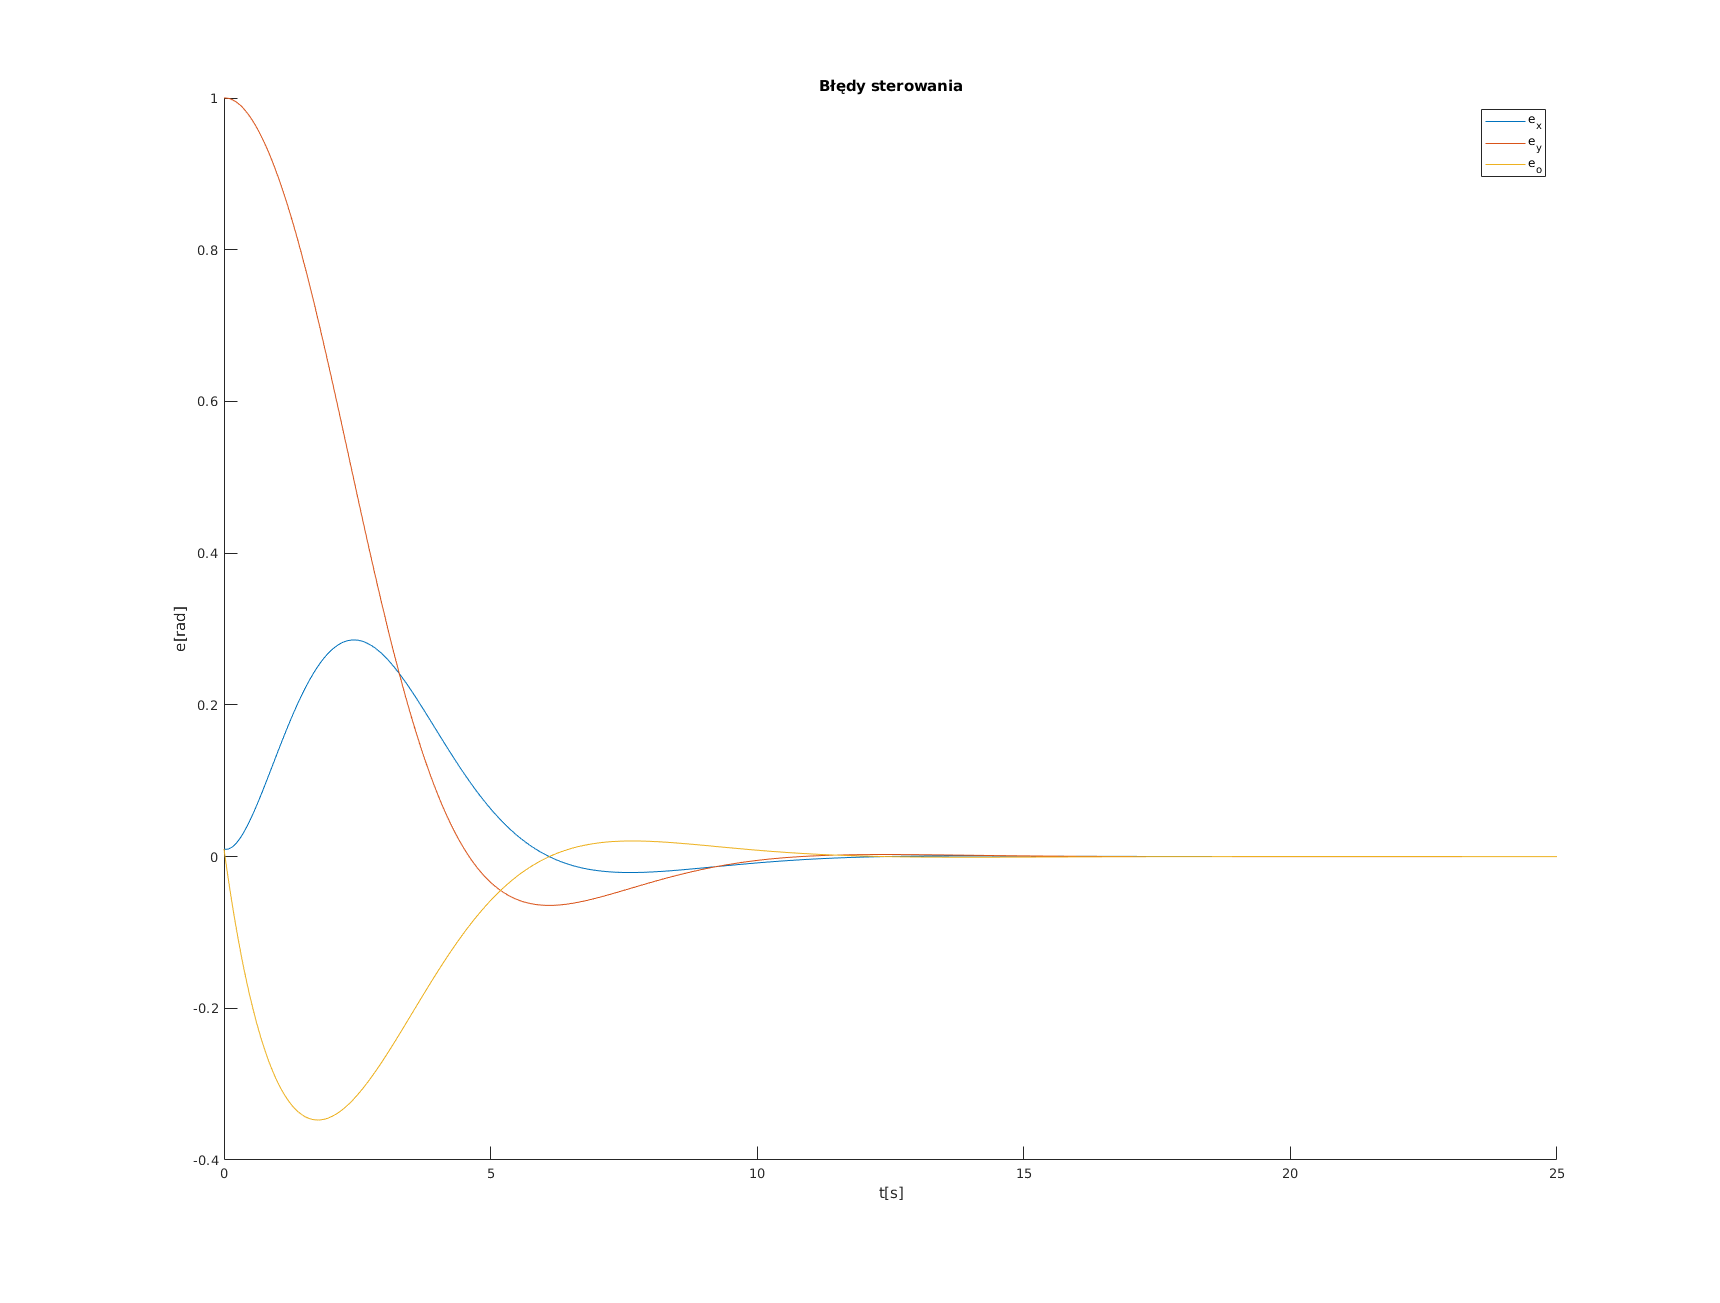
\includegraphics[width=1\textwidth]{figures/kin_bledy.png}
    \caption{Błędy $e_x$, $e_y$, $e_\theta$}
    \label{fig:1}
  \end{figure}

  \begin{figure}[H]
    \centering
    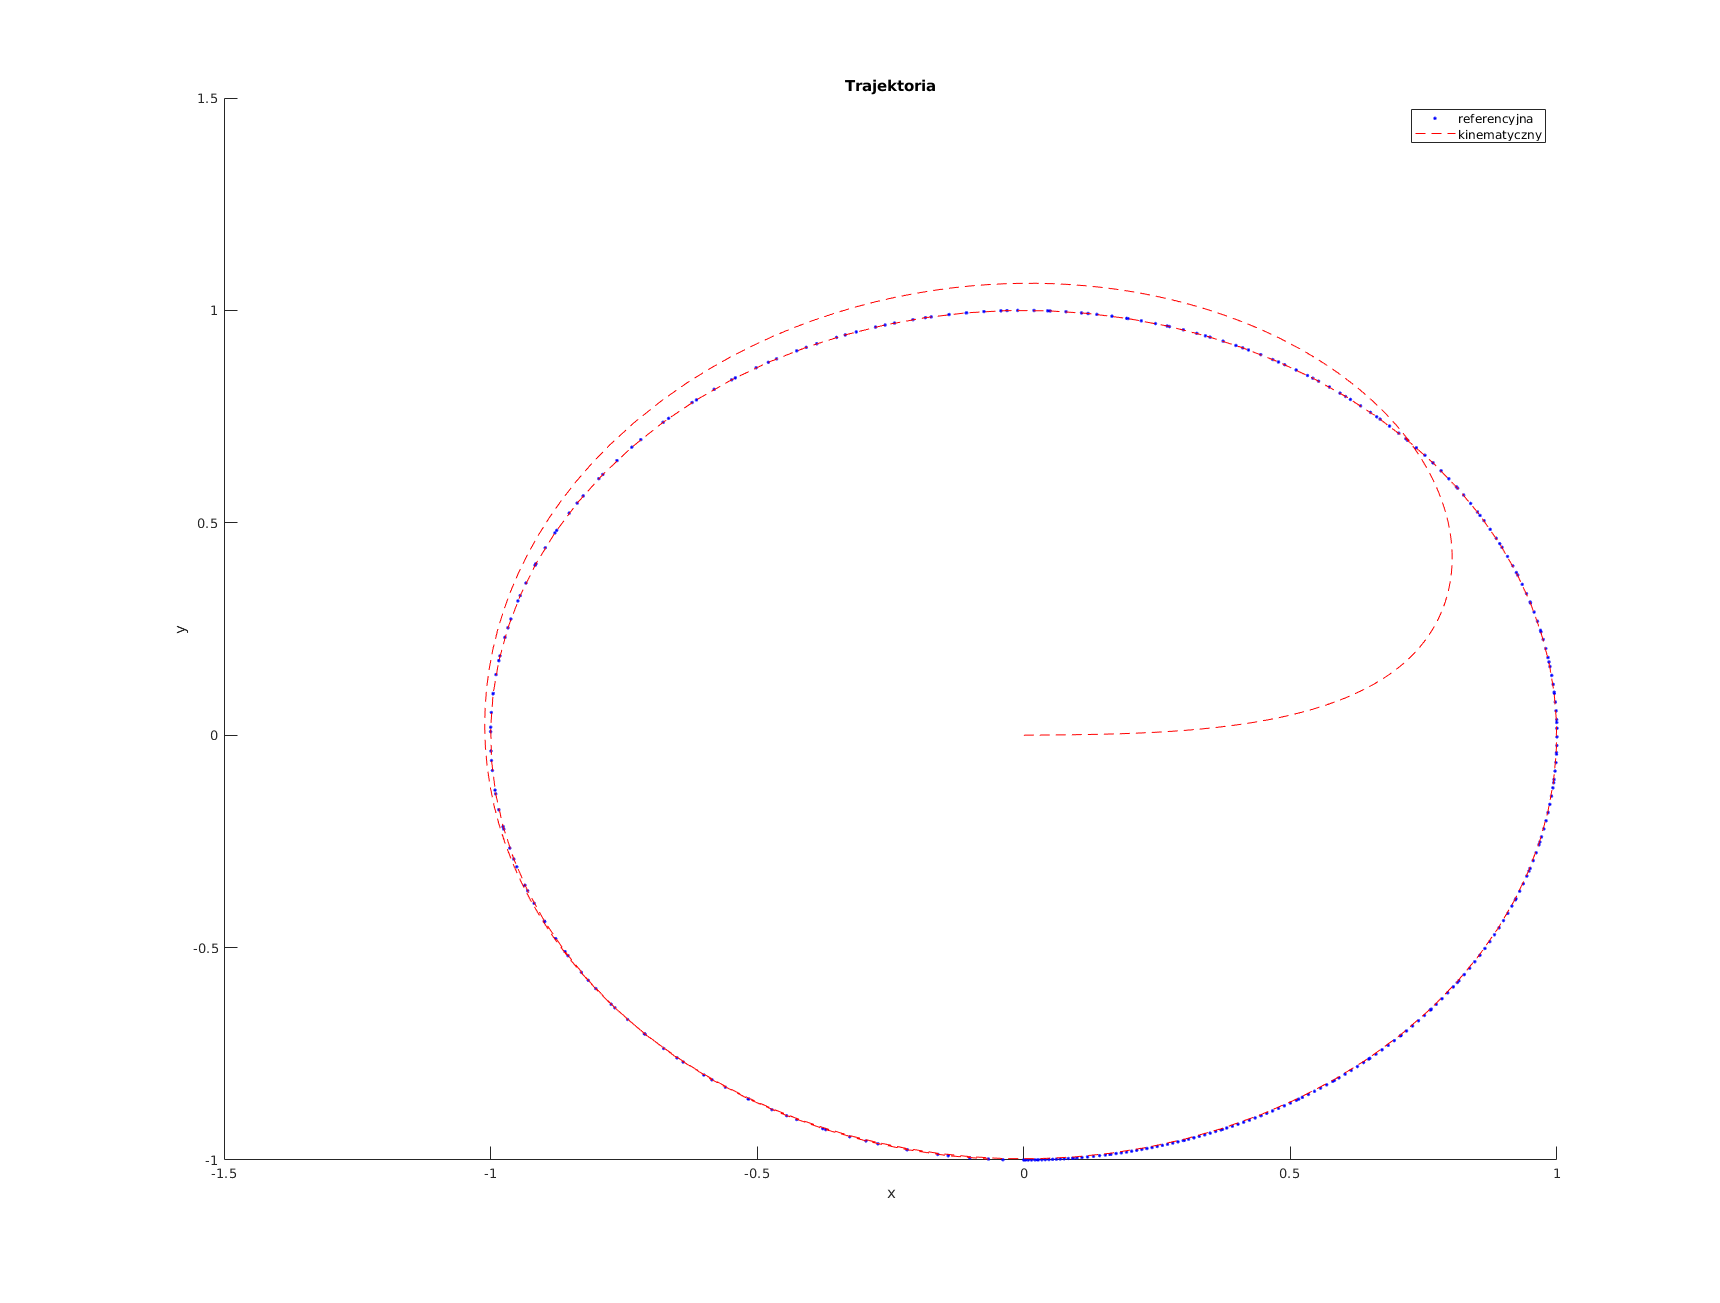
\includegraphics[width=1\textwidth]{figures/kin_trajektoria.png}
    \caption{Trajektoria}
    \label{fig:2}
  \end{figure}


\section{Sterownik kinematyczny i dynamiczny}

  \subsection{Błędy śledzenia trajektorii}
    Eksperyment ten zakłada wykorzystanie dwóch sterowników kinematycznego i dynamicznego jednocześnie. Profil prędkościowy produkowany przez sterownik kinematyczny jest wykorzystywany przez sterownik dynamiczny, którego zadaniem jest minimalizacja błędów śledzenia trajektorii.

    \begin{figure}[H]
      \centering
      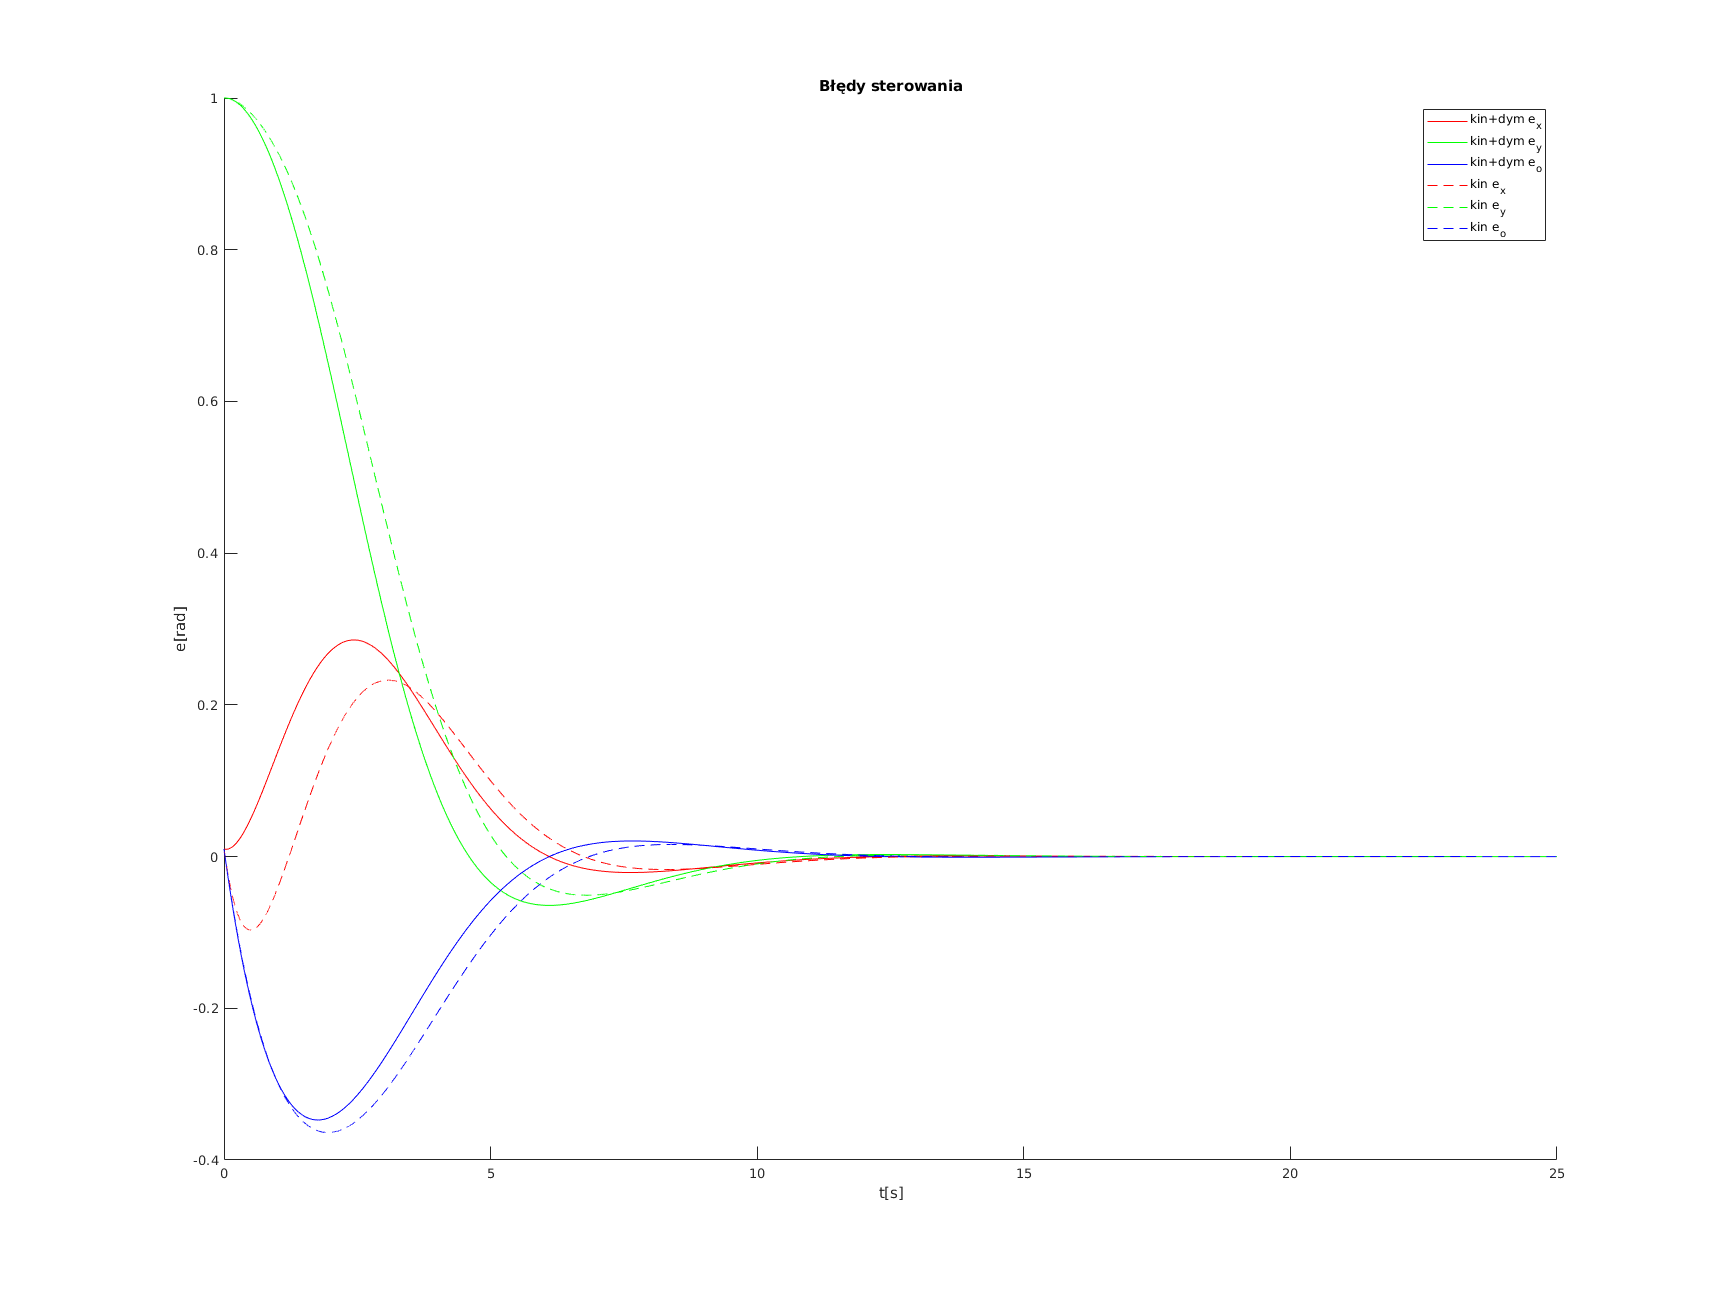
\includegraphics[width=1\textwidth]{figures/dyn_bledy.png}
      \caption{Błędy $e_x$, $e_y$, $e_\theta$}
      \label{fig:3}
    \end{figure}

    Na wykresie \ref{fig:3} można zaobserwować odnotowane błędy śledzenia trajektorii. Liniami ciągłymi oznaczone są błędy dotyczące sterownika kinematycznego, natomiast liniami przerywanymi rysowane są wykresy dotyczące połączenia oby sterowników. Ciężko jest jednocześnie stwierdzić że połączenie obu sterowników daje wymiernie lepsze efekty. Zdecydowanie wprowadza ono pewne opóźnienie, ale w tym konkrentym przypadku da się zauważyć że wprowadza ono nieznacznie mniejsze przesterowania. 

    \begin{figure}[H]
      \centering
      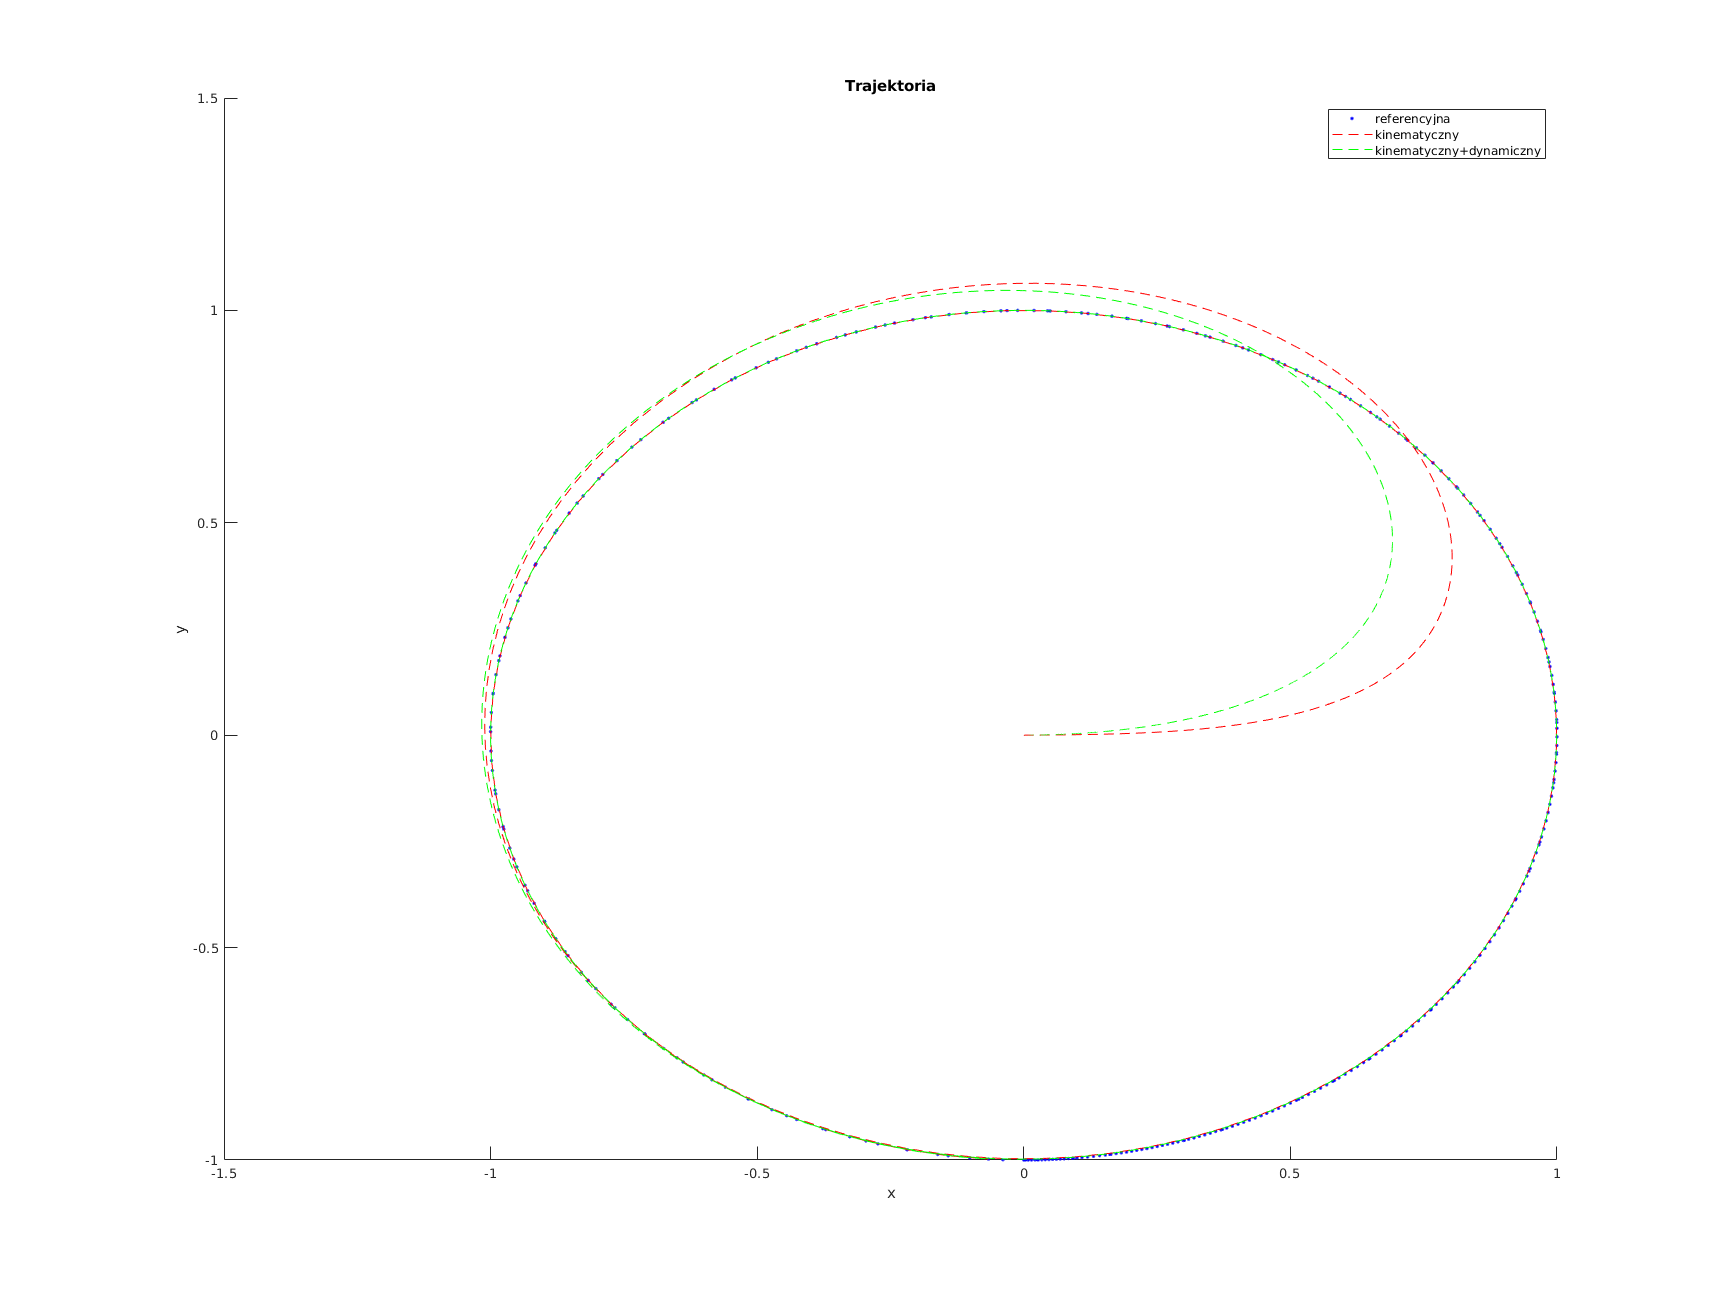
\includegraphics[width=1\textwidth]{figures/dyn_trajektoria.png}
      \caption{Trajektoria}
      \label{fig:4}
    \end{figure}

    Wykres \ref{fig:4} porównuje trajektorie referencyjną do trajektorii ze sterownikiem dynamicznym oraz bez sterownika dynamiczengo. Dodanie sterowanika dynamicznego spowodowało bardziej zdecydowaną reakcję obiektu w początkowej fazie ruchu porównując z drugim mniej skomplikowanym rozwiązaniem. Jednakże czas potrzebny na osiągniecie zadanej trajektorii jest bardzo porównywalny. 

  \subsection{Zależność od współczynnika $K_1$}
  Wykres \ref{fig:5} przedstawia jak wpływa zmiana współczynnika $K_1$ na poszczególne błędy śledzenia, przy zachowaniu współczynnika $K_2$ równemu 1. Na podstawie tych danych można wywnioskować że wzrost wzmocnienia $K_1$:

  \begin{itemize}
    \item znacznie zmniejsza błąd $E_x$ oraz skraca jego czas stabilizacji,
    \item powoduje mniej stromy spadek błędów $E_y$ oraz $E_\theta$ i wydłuża ich czas stabilizacji, niwelując przesterowania.
  \end{itemize}
  
  \begin{figure}[H]
    \centering
    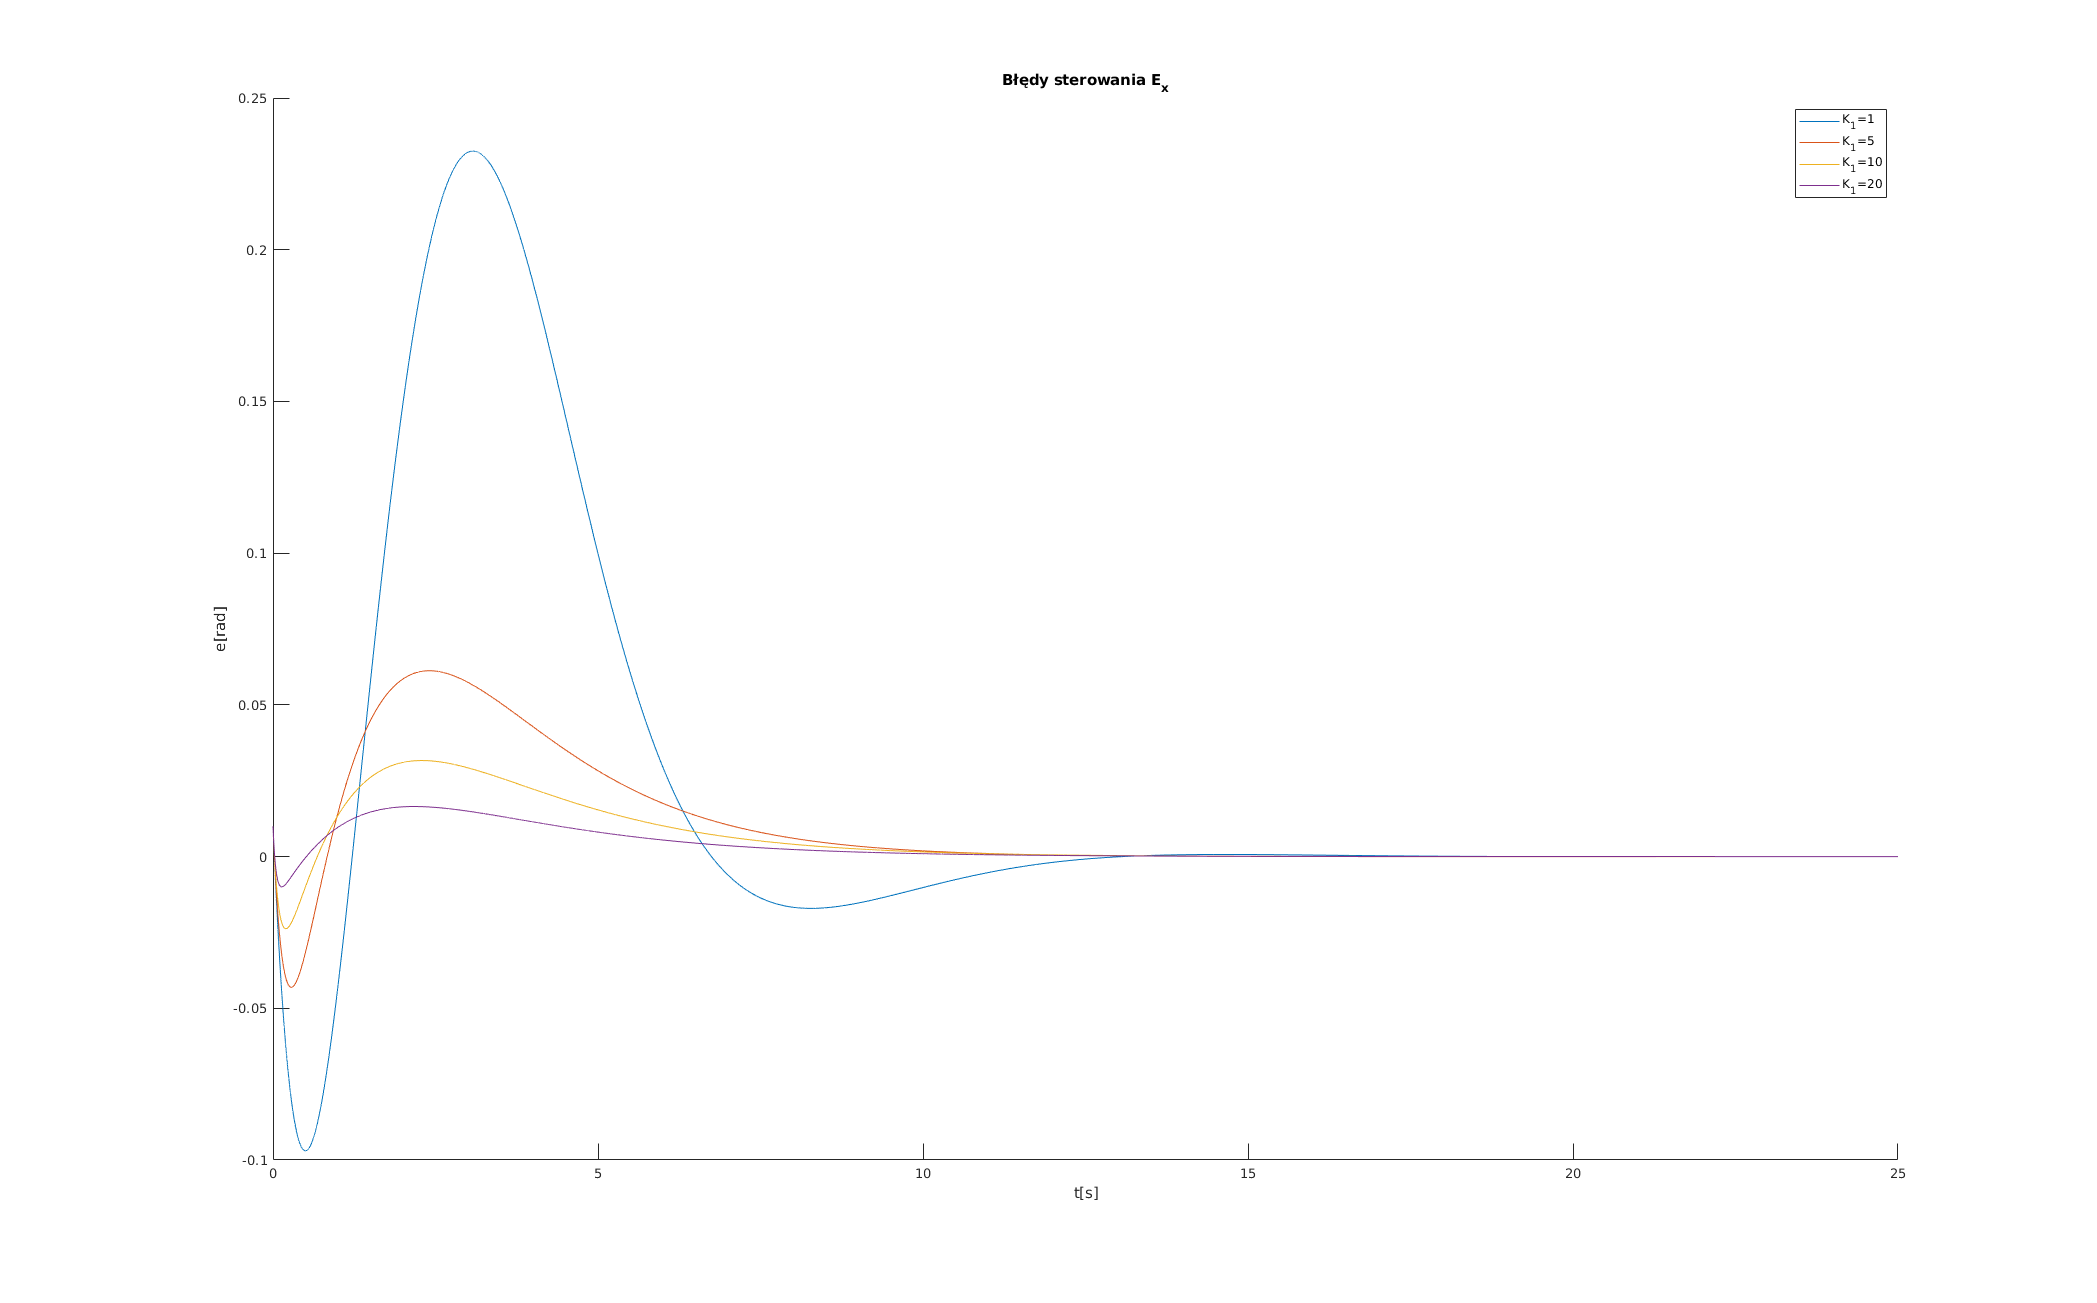
\includegraphics[height=0.3\textheight]{figures/dyn_bledy_k1_ex.png}
    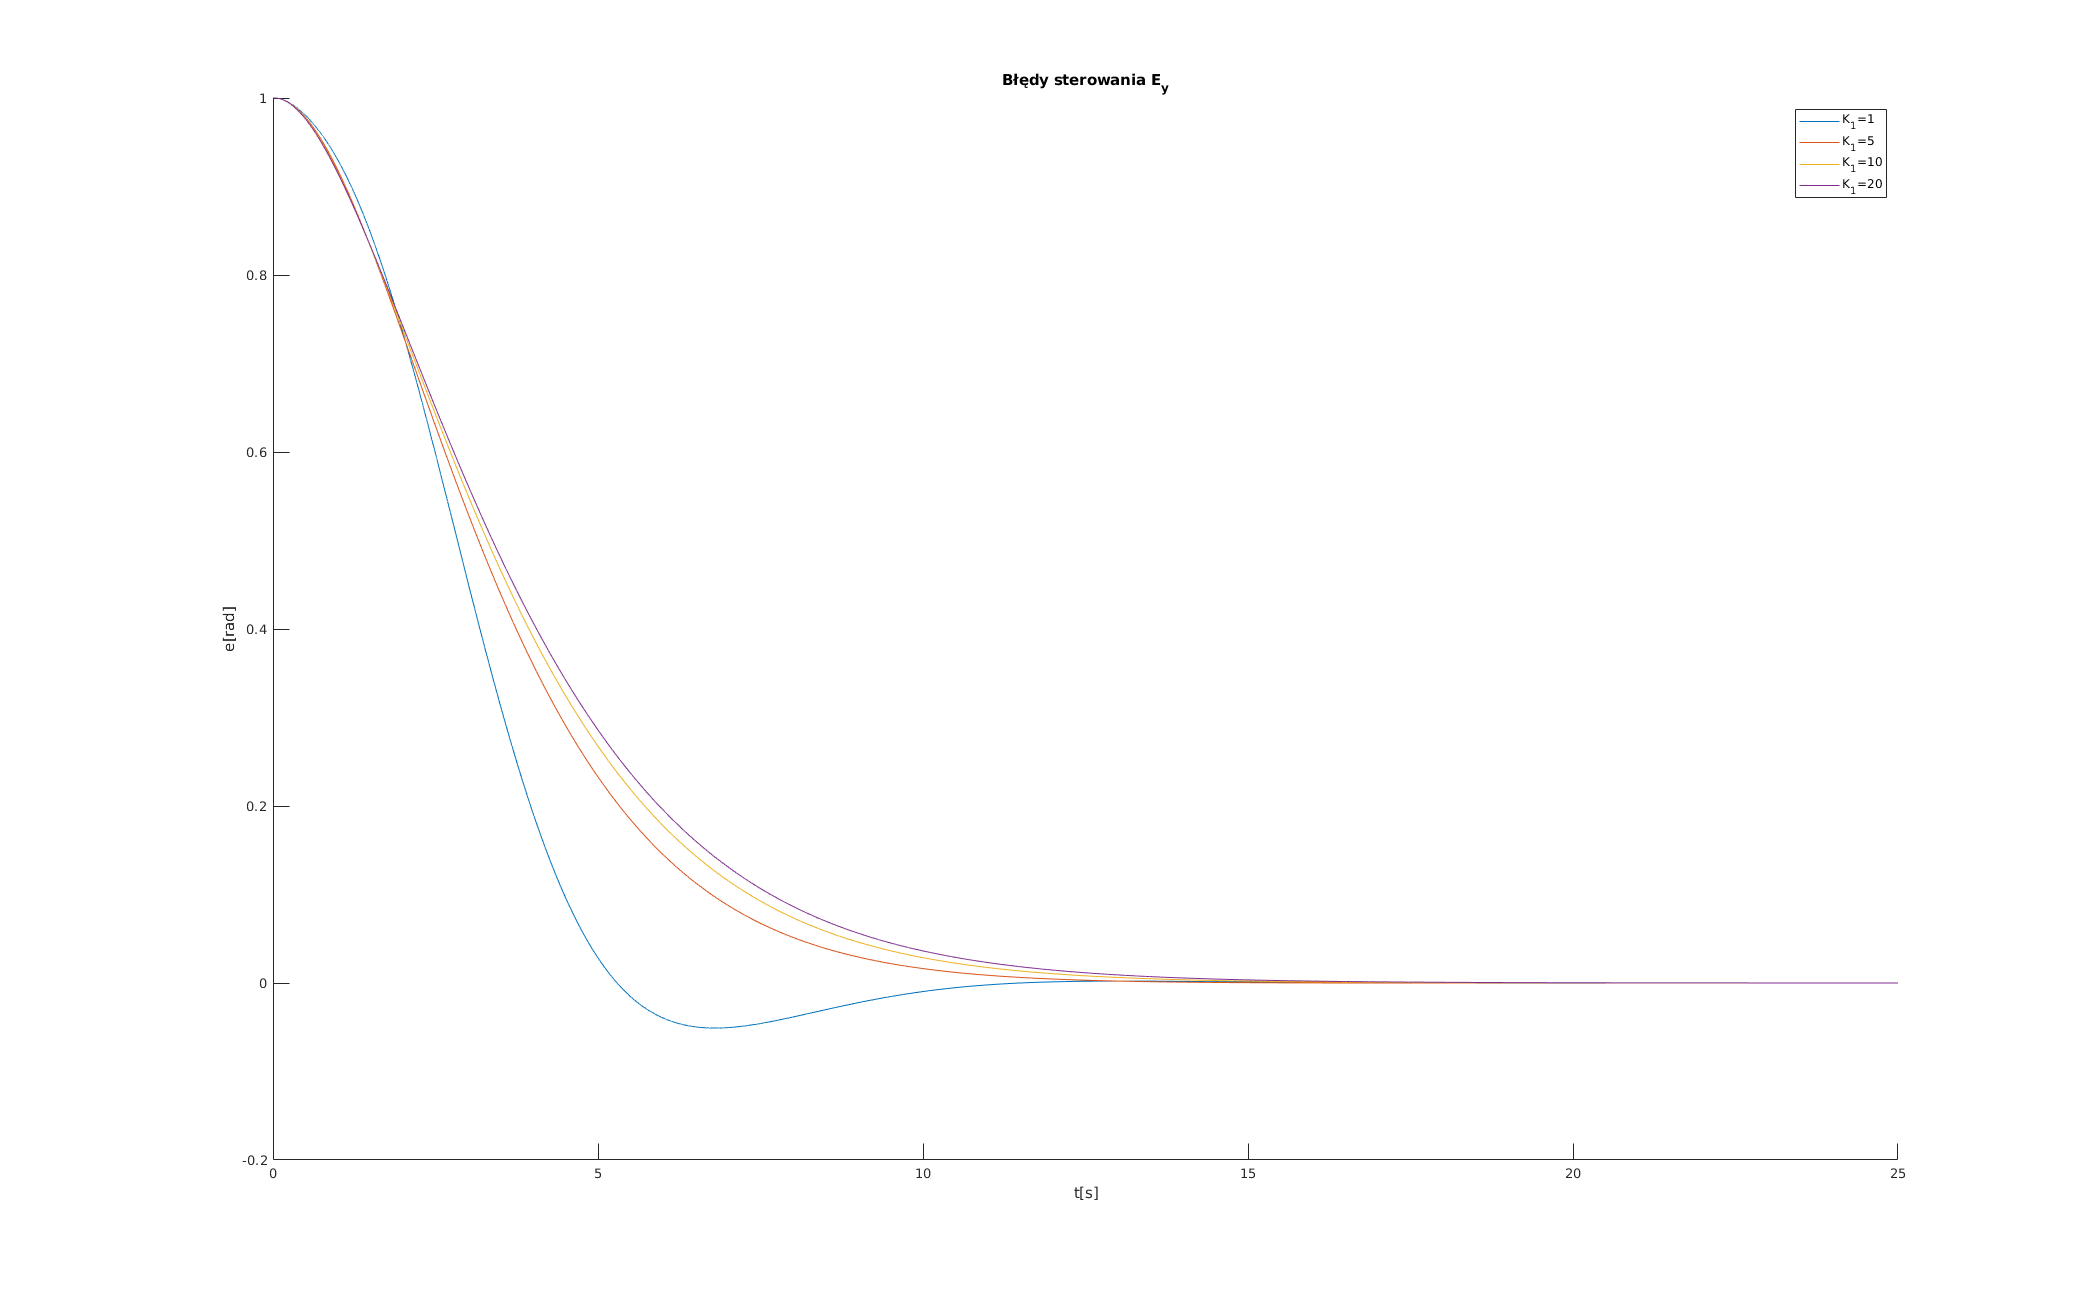
\includegraphics[height=0.3\textheight]{figures/dyn_bledy_k1_ey.png}
    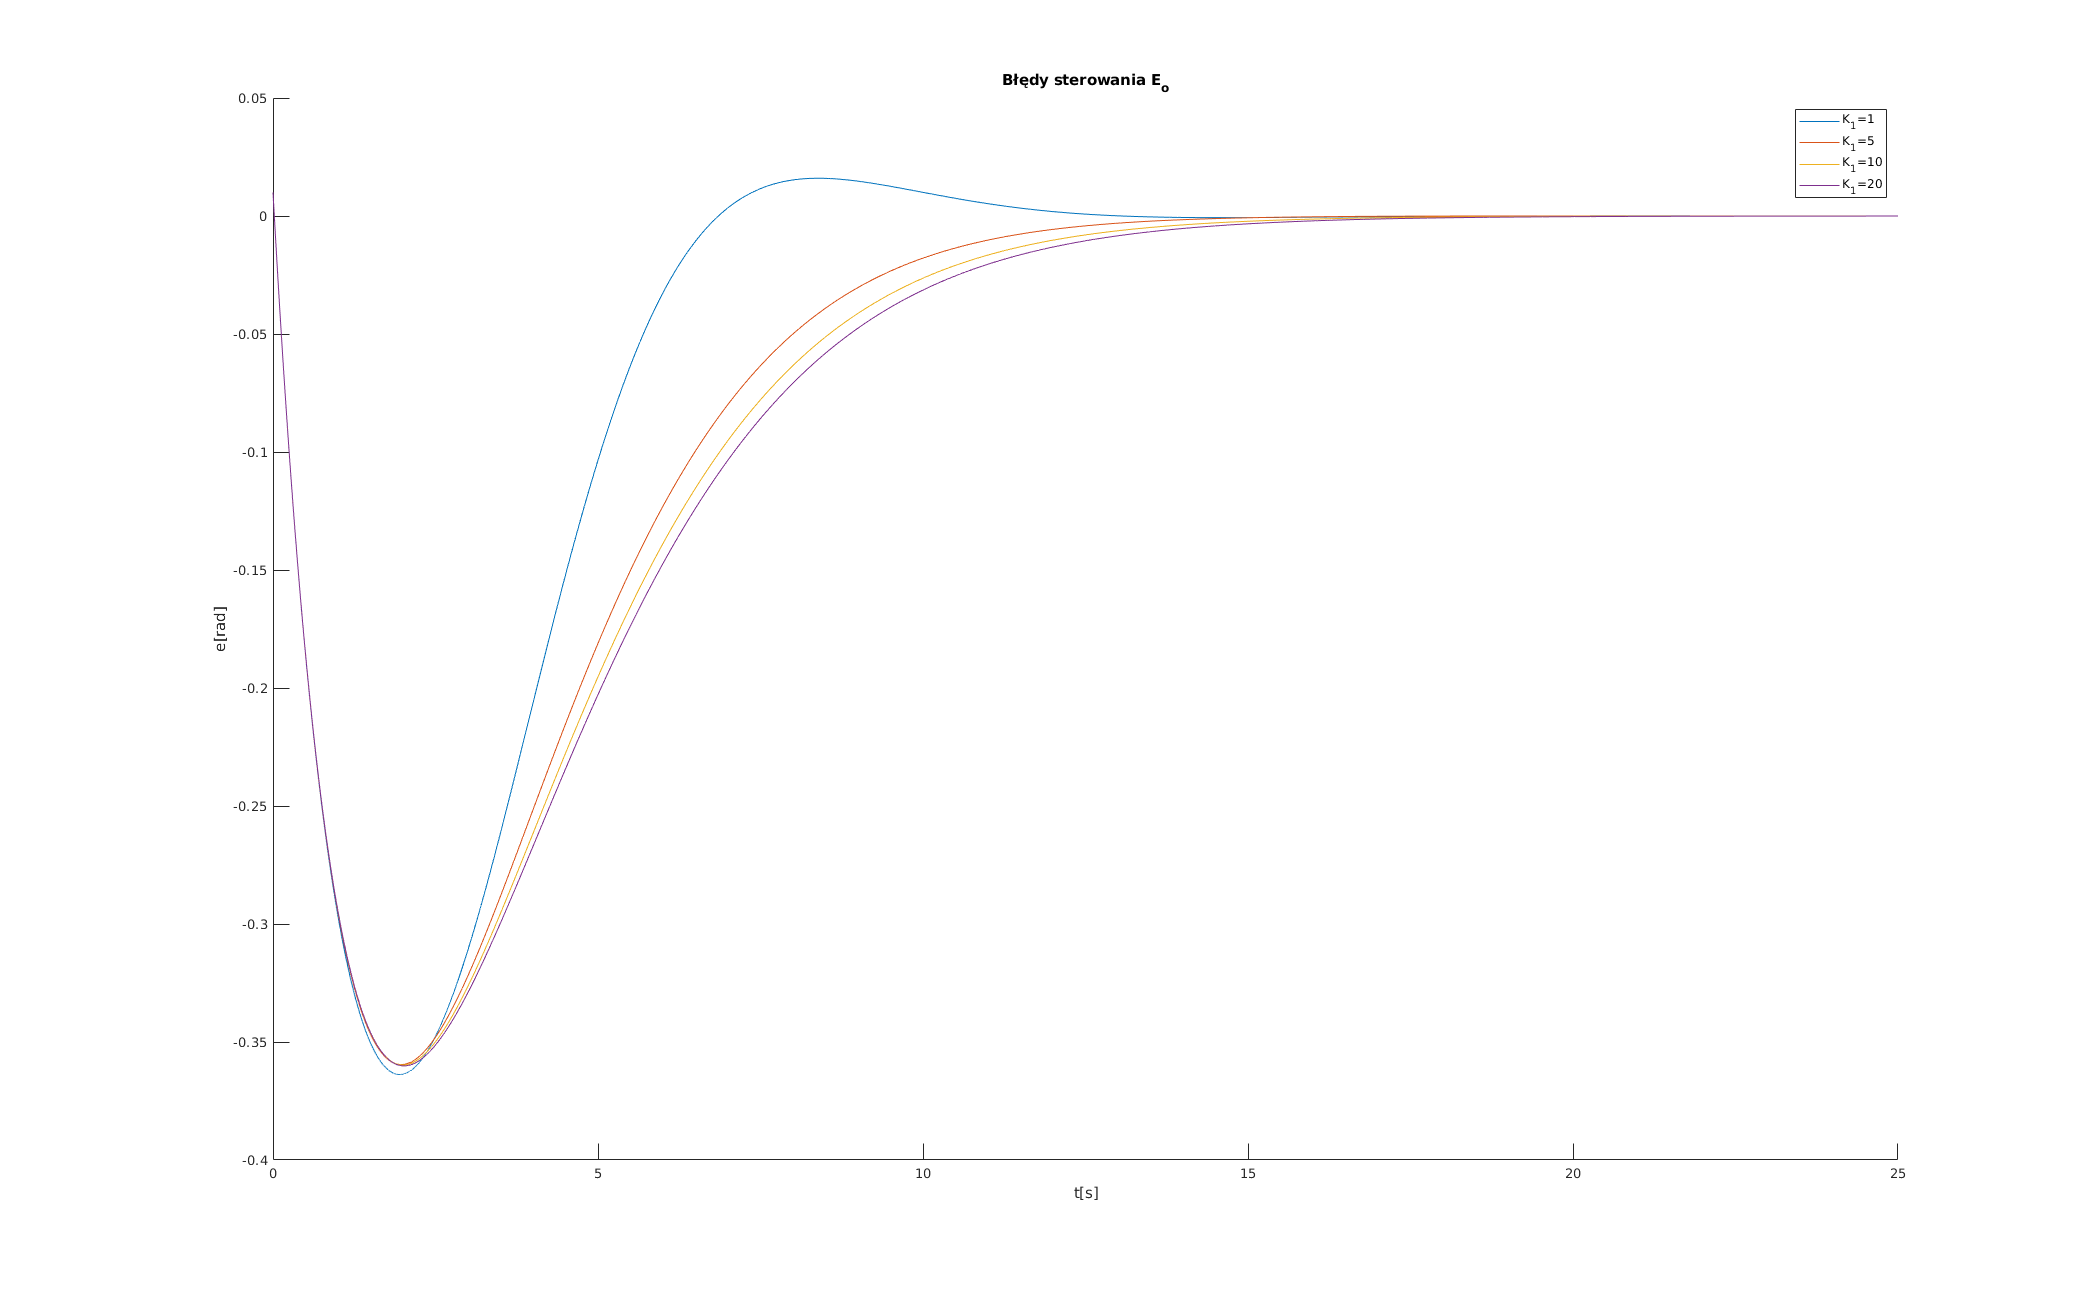
\includegraphics[height=0.3\textheight]{figures/dyn_bledy_k1_eo.png}
    \caption{Błędy $e_x$, $e_y$, $e_\theta$}
    \label{fig:5}
  \end{figure}




  \subsection{Zależność od współczynnika $K_2$}
  Wykres \ref{fig:6} przedstawia jak wpływa zmiana współczynnika $K_2$ na poszczególne błędy śledzenia, przy zachowaniu współczynnika $K_1$ równemu 1. Na podstawie tych danych można wywnioskować że wzrost wzmocnienia $K_2$:

  \begin{itemize}
    \item znacznie zmniejsza błąd $E_\theta$ oraz skraca jego czas stabilizacji,
    \item powoduje mniej stromy spadek błędów $E_x$ oraz $E_y$ i wydłuża ich czas stabilizacji, niwelując przesterowania.
  \end{itemize}
  
  \begin{figure}[H]
    \centering
    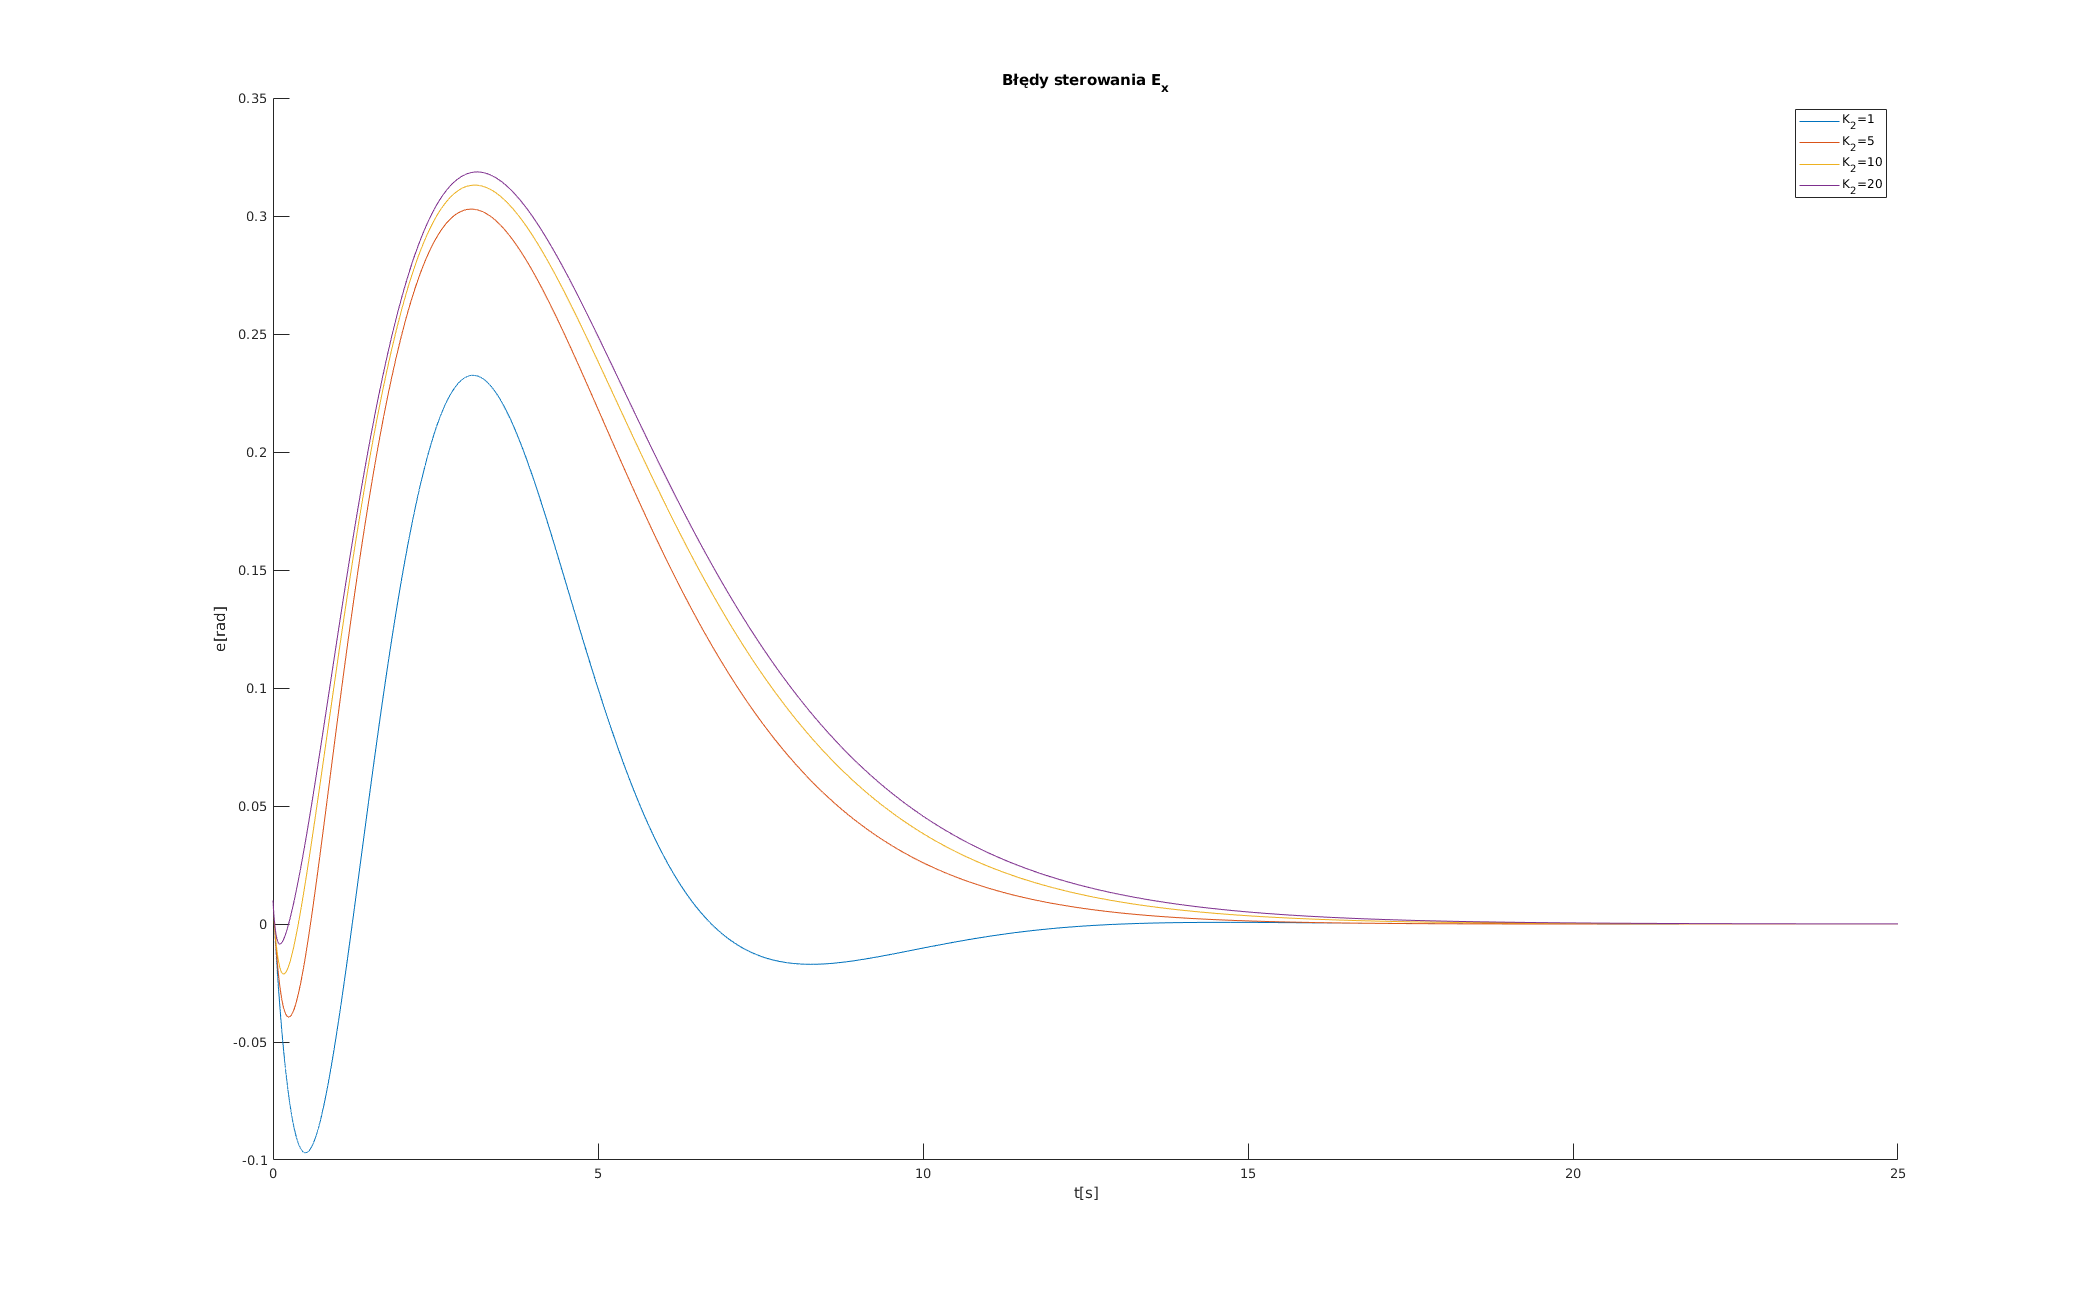
\includegraphics[height=0.3\textheight]{figures/dyn_bledy_k2_ex.png}
    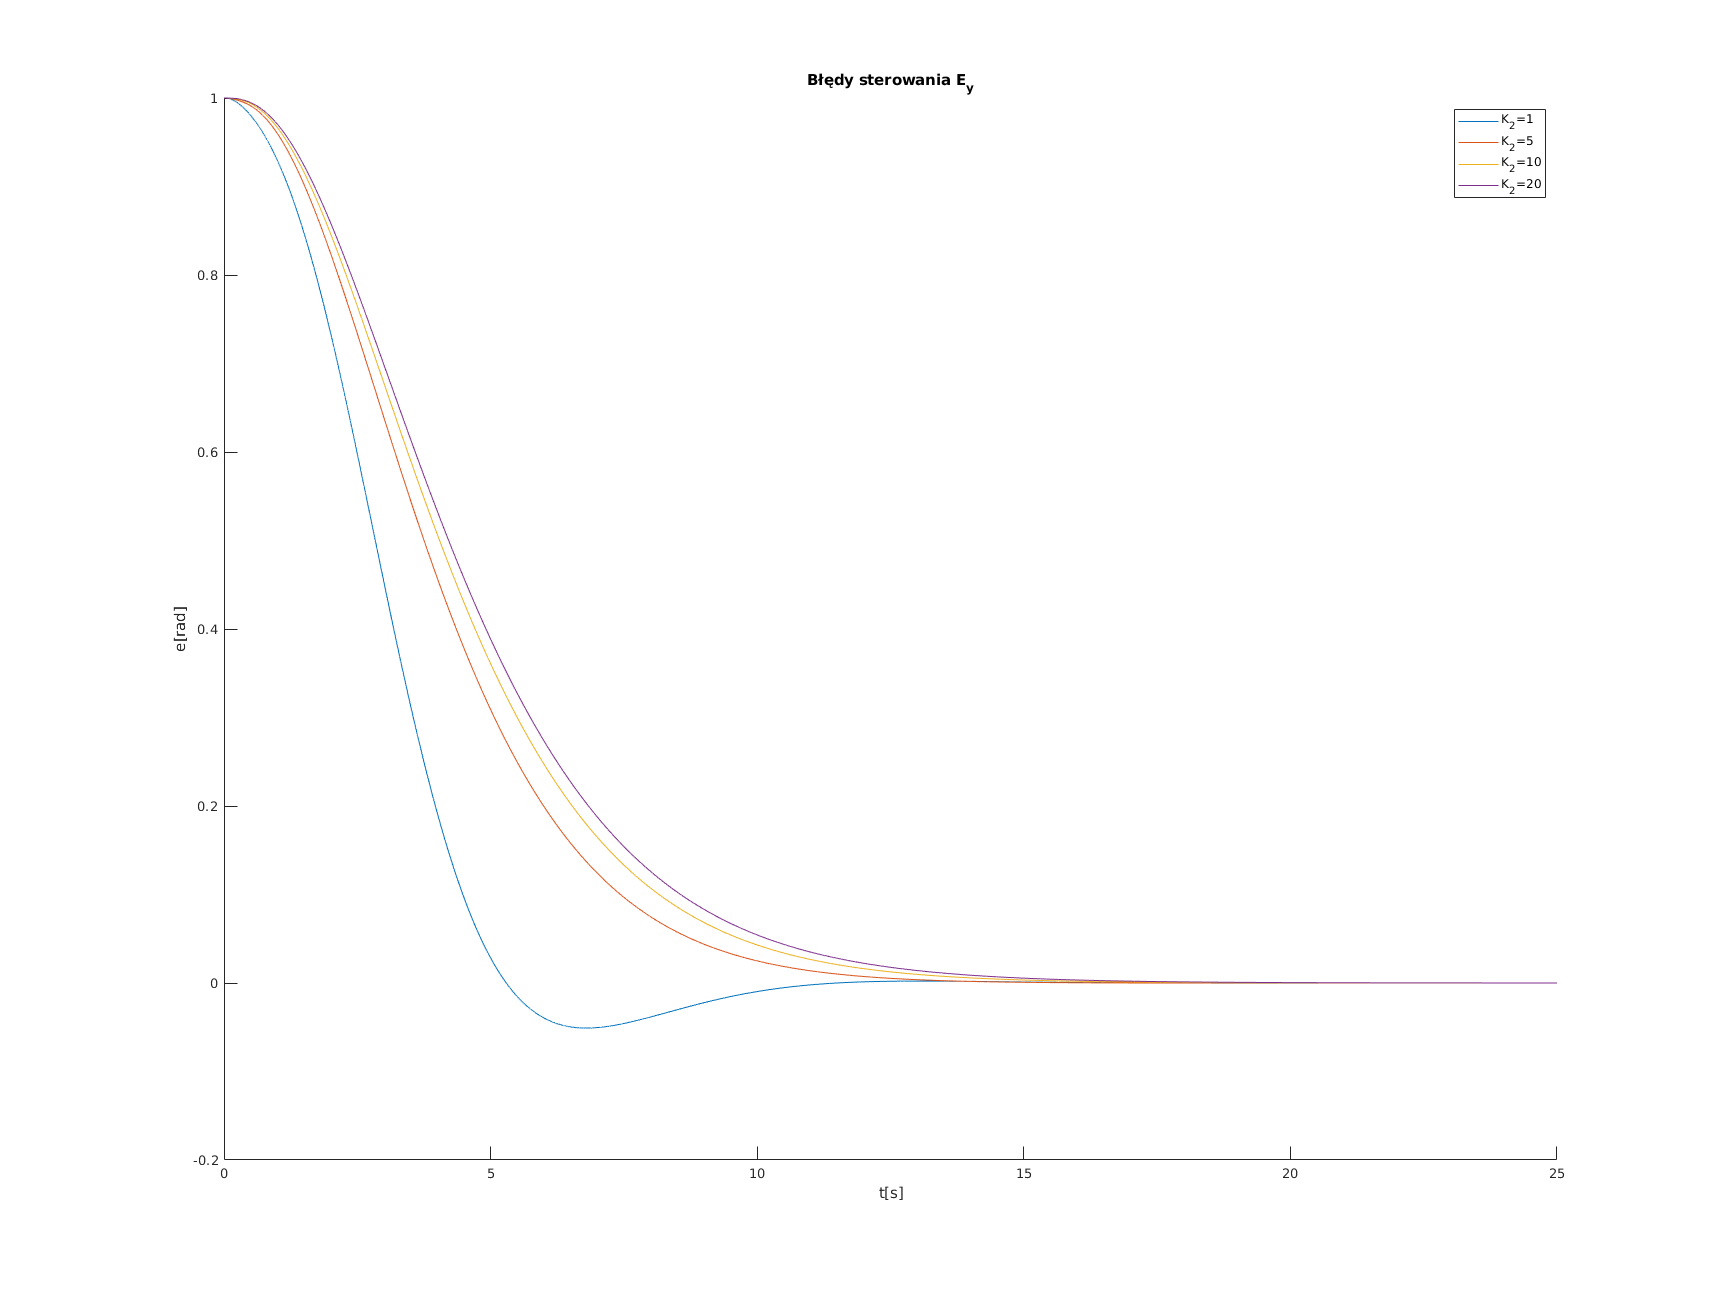
\includegraphics[height=0.3\textheight]{figures/dyn_bledy_k2_ey.png}
    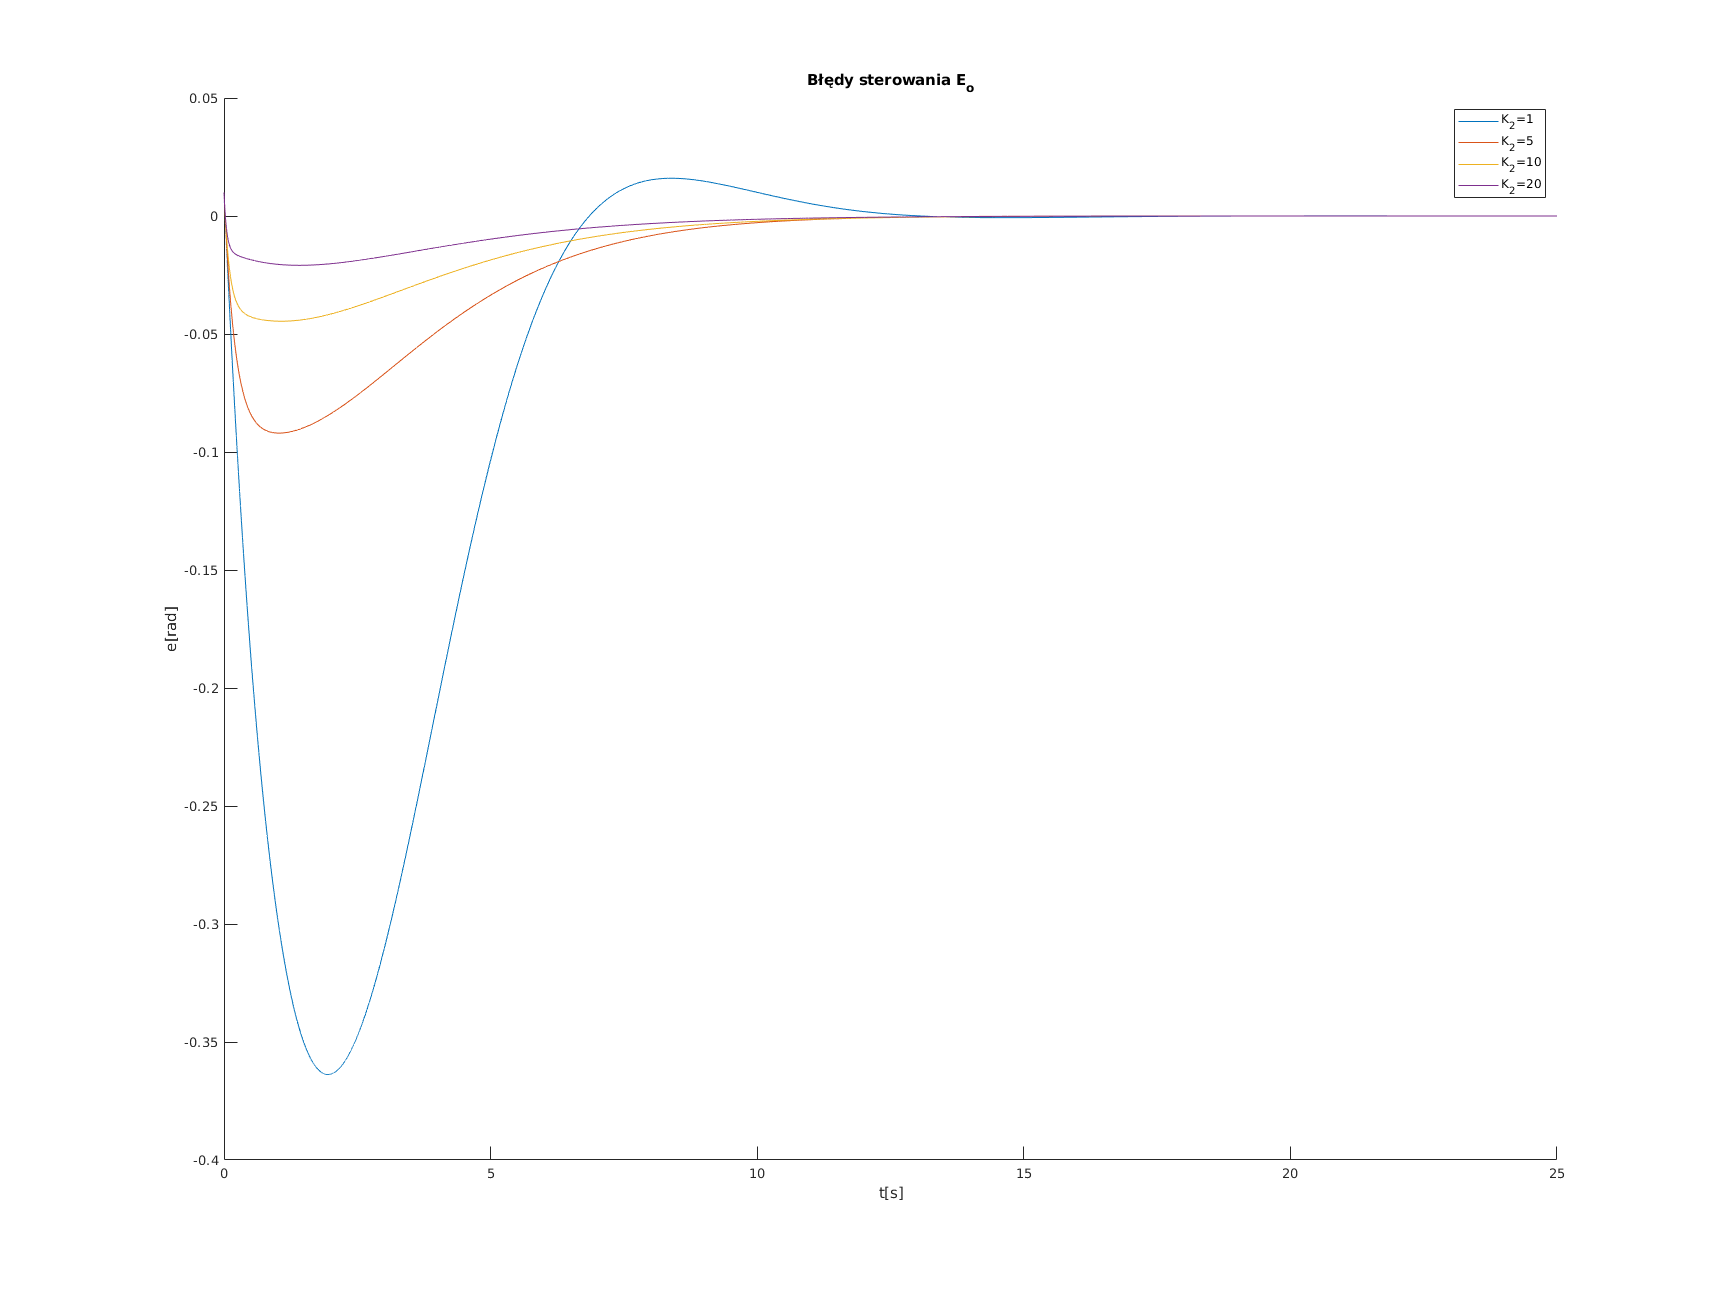
\includegraphics[height=0.3\textheight]{figures/dyn_bledy_k2_eo.png}
    \caption{Błędy $e_x$, $e_y$, $e_\theta$}
    \label{fig:6}
  \end{figure}




  \subsection{Zależność od współczynnika $K_M$}

  % Symulacje przeprowadzono przy stałym wzmocnieniu K0 wynoszącym 1 oraz zmianie parametru K1.

  % \begin{figure}[H]
  %   \centering
  %   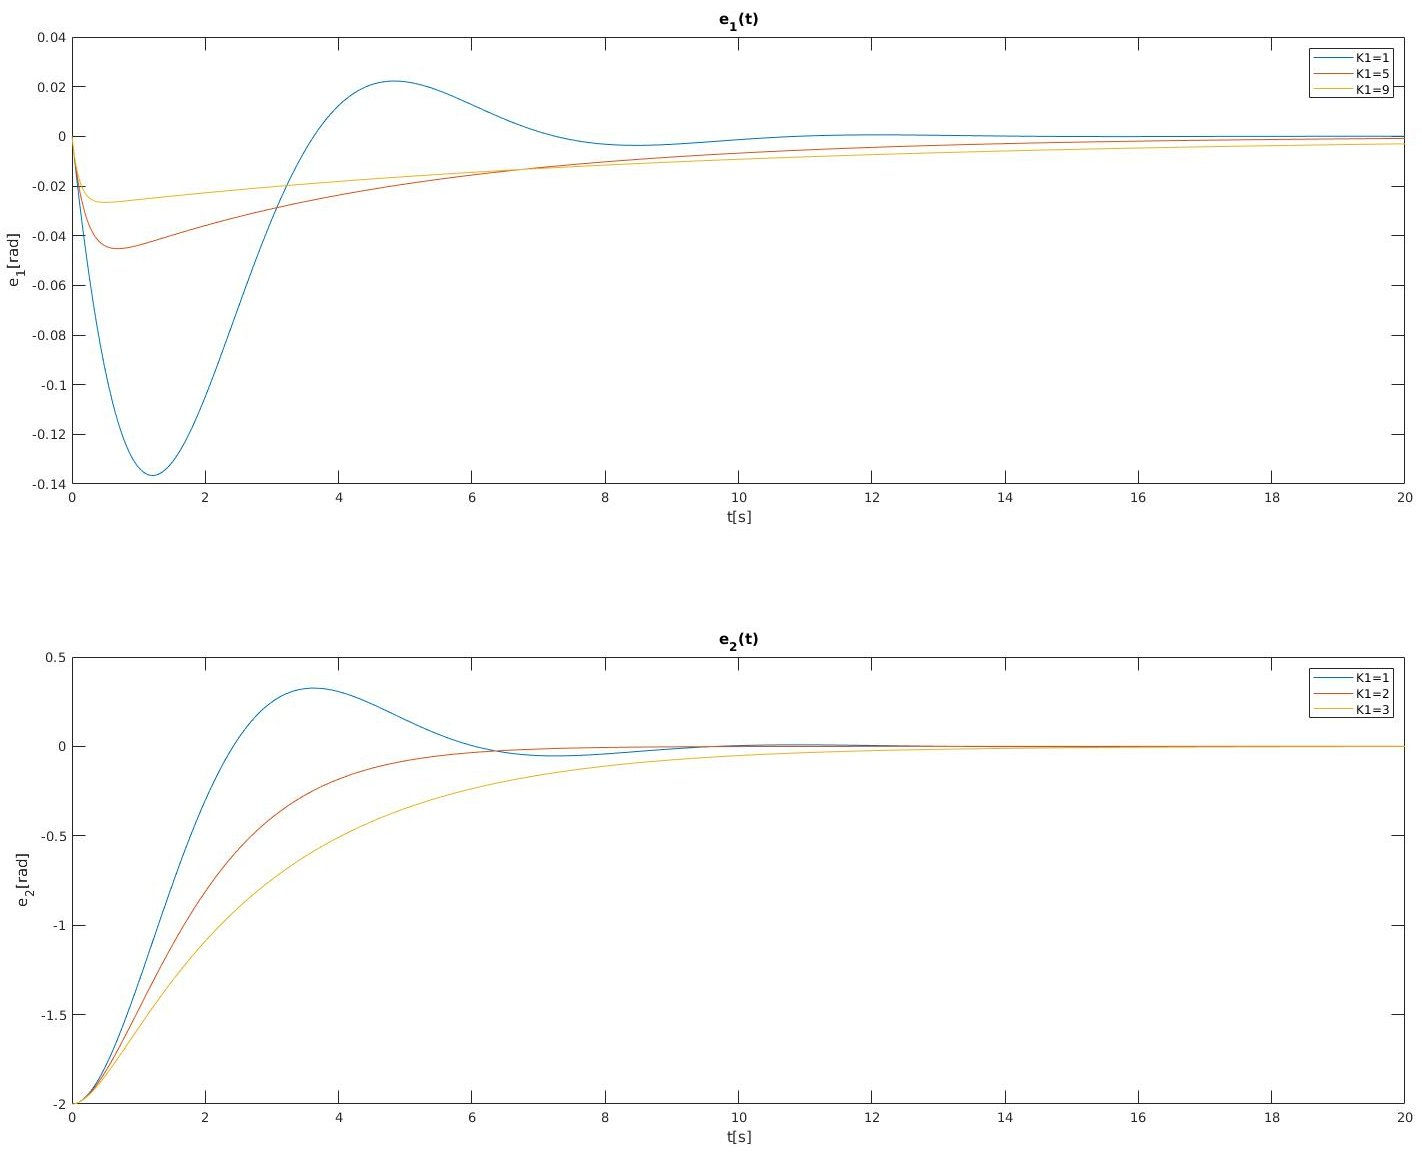
\includegraphics[width=1\textwidth]{figures/lin2.jpg}
  %   \caption{stałe K0 = 1, zmienne K1}
  %   \label{fig:lin2}
  % \end{figure}

  % \begin{table}[h!]
  %   \centering
  %   \begin{tabular}{ r | c | c }
  %     K1 & Przesterowanie $e_1$ [rad] & Czas wygaszania $e_1$ \\ 
  %     \hline
  %     1 & $15.87 \cdot 10^{-2}$ & 8  \\
  %     5 & $4.52  \cdot 10^{-2}$ & 12   \\
  %     9 & $2.64  \cdot 10^{-2}$ & 16
  %   \end{tabular}
  %   \caption{Charakterystyka przebiegów błędu $e_1$ w zależności od K1.}
  %   \label{table:4}
  % \end{table}

  %   Wzrost wzmocnienia K1 powoduje spadek przesterowania przegubu pierwszego. Negatywnym skutkiem takich nastaw jest wydłużony czas wygaszania oscylacji (patrz tabela \ref{table:4}).

  % \begin{table}[h!]
  %   \centering
  %   \begin{tabular}{ r | c | c }
  %     K1 & Przesterowanie $e_2$ [rad] & Czas wygaszania $e_2$ [s]  \\ 
  %     \hline
  %     1 & $37.8 \cdot 10^{-2}$ & 12 \\
  %     2 & $1.41 \cdot 10^{-6}$ & 8  \\
  %     3 & $2.36 \cdot 10^{-3}$ & 15
  %   \end{tabular}
  %   \caption{Charakterystyka przebiegów błędu $e_2$ w zależności od K1.}
  %   \label{table:5}
  % \end{table}

  %   Najlepsze zachowanie przegubu drugiego zaobserwowano dla wzmocnienia $K1=2$ (patrz tabela \ref{table:5}).


  % \subsection{Zależność od wartości początkowej}

  %   Rysunek \ref{fig:lin3} przedstawia przebiegi błędów śledzenia trajektorii w zależności od różnych punktów startowych.

  % \begin{figure}[H]
  %   \centering
  %   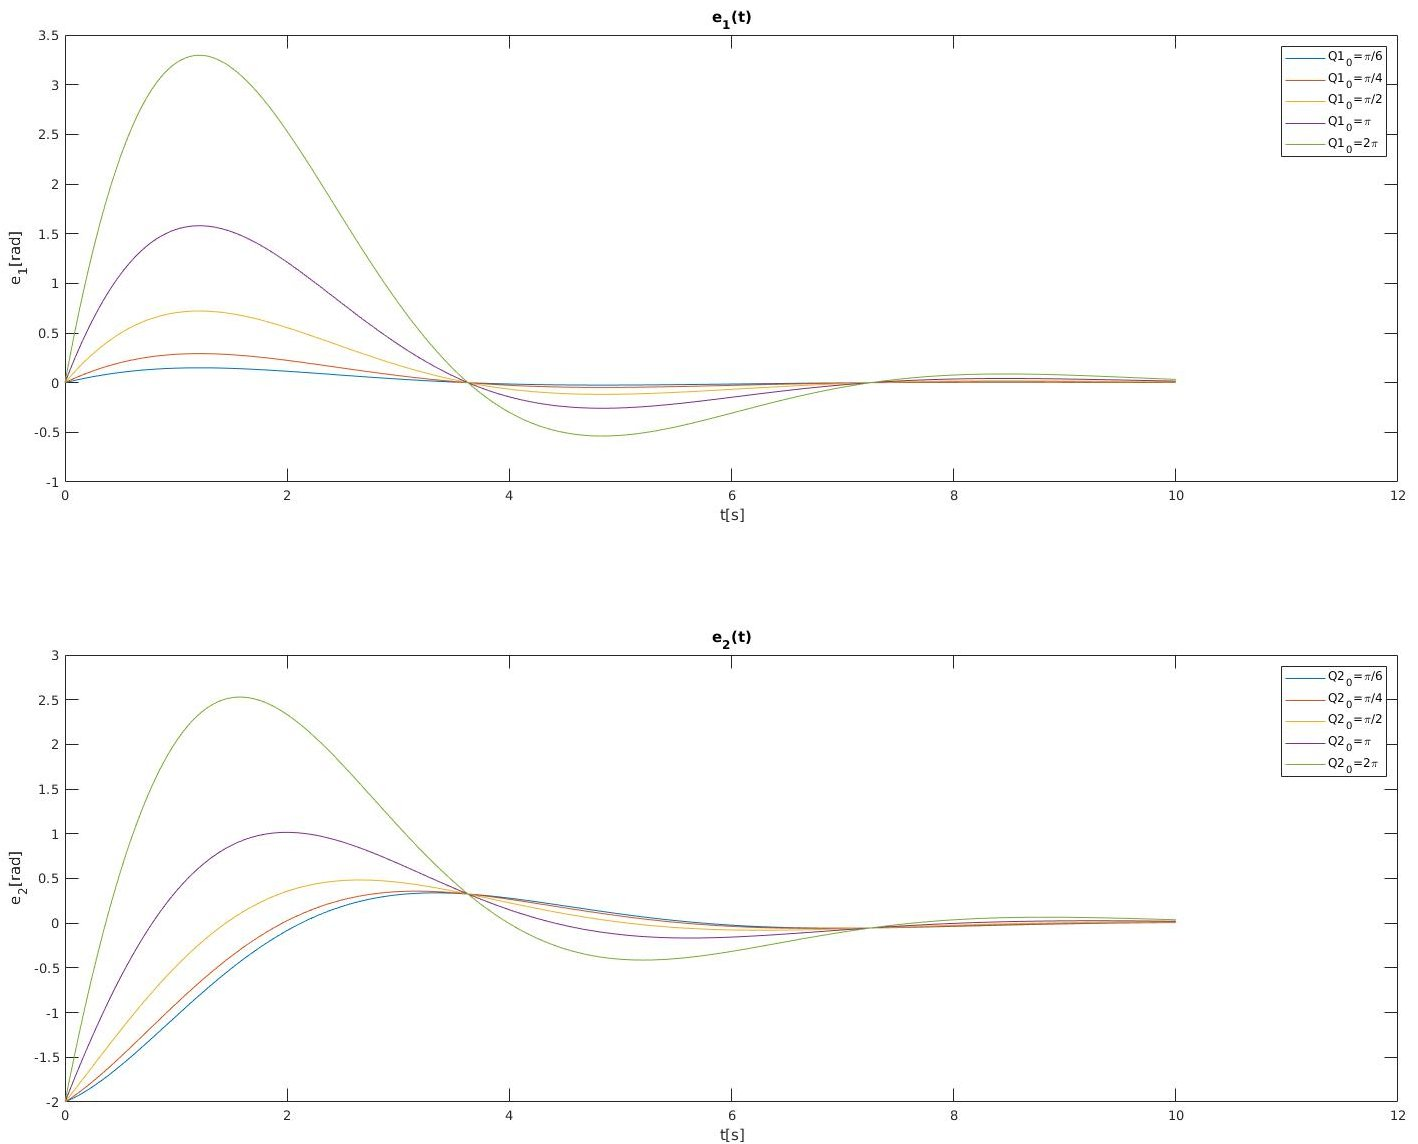
\includegraphics[width=1\textwidth]{figures/lin3.jpg}
  %   \caption{Charakterystyka przebiegów błędu w zależności od położenia początkowego.}
  %   \label{fig:lin3}
  % \end{figure}

  %   Pierwsza część wykresu \ref{fig:lin3} dotyczy zmiany położenia pierwszego przegubu. Im przegub startuje z miejsca bardziej oddalonego od punktu zerowego tym większy błąd początkowy i dłuższy czas stabilizacji. Druga część wykresu odpowiada za drugi przegób. W tym przypadku również większe wychylenia powodują identyczne skutki, jak w pierwszym przegubie.

  % \begin{figure}[H]
  %   \centering
  %   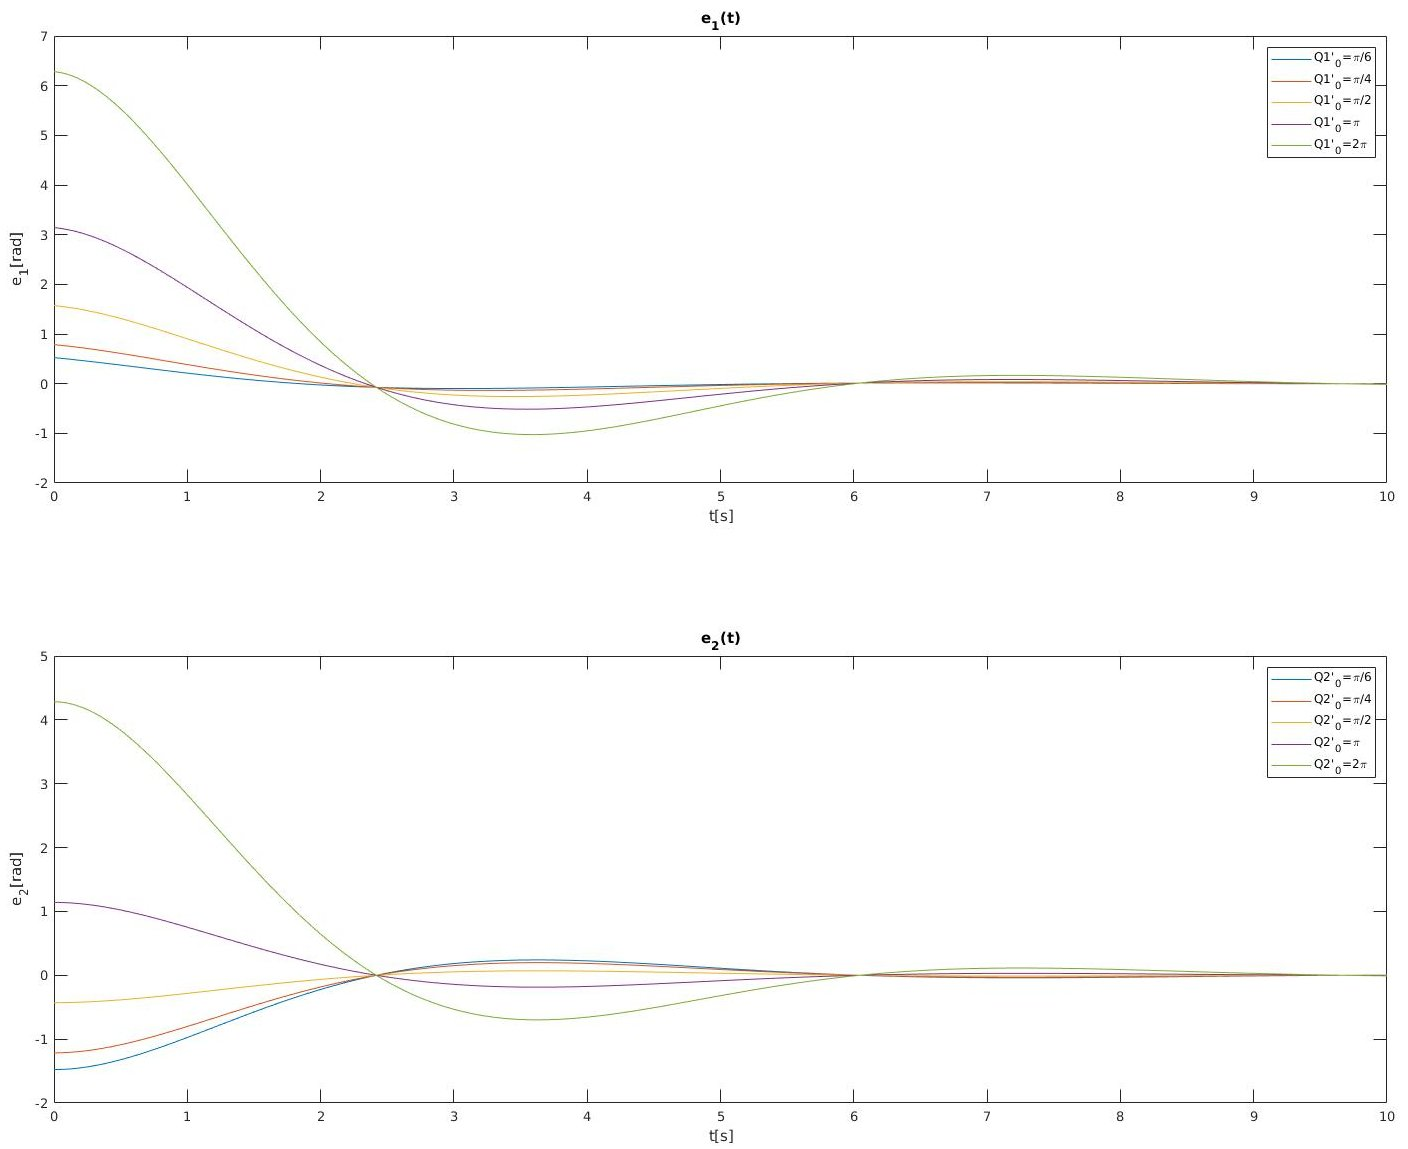
\includegraphics[width=1\textwidth]{figures/lin4.jpg}
  %   \caption{Charakterystyka przebiegów błędu w zależności od prędkości początkowej.}
  %   \label{fig:lin4}
  % \end{figure}

  %   Wykres \ref{fig:lin4} prezentuje jaki wpływ na błąd śledzenia ma prędkość początkowa. W górnej części poświęconej przegubowi pierwszemu, zwiększanie prędkości początkowej powoduje coraz to większe przesterowania. Dolna część dotycząca drugiego przegubu przy pewnej prędkości początkowej ma dużo mniejszy błąd niż przy starcie ze stanu spoczynku. Jest to spowodowane tym że odpowiednio rozpędzony przegób może szybciej znaleźć się w zadanym położeniu. Intuicyjne jest również to że przy zbyt wielkiej prędkości błąd znów zacznie rosnąć. 
    
  \subsection{Zależność od warunków początkowych}

  wykresy błędów Ex, Ey, Eo
  wykres trajektorii



  \subsection{Wnioski}
  dlaczego dla platformy musi być kinematyczny i dynamiczny i skąd to się wzięło

  % \begin{itemize}
  %   \item wzrost wzmocnienia K0 powoduje zwiększone przesterowanie i wydłużony czas tłumienia oscylacji dla obu przegubów,
  %   \item wzrost wzmocnienia K1 powoduje spadek przesterowania i wydłużony czas tłumienia oscylacji dla przegubu pierwszego,
  %   \item dla przegubu drugiego ustawienie wzmocnienienia $K1=2$ spowodowało osiągnięcie najlepszych rezultatów,
  %   \item położenie i prędkość początkowa mają duże znaczenie na błąd w pierwszych sekundach sterowania. 
  % \end{itemize}
  
\section{Podsumowanie}
  Algorytm Qui Dorsey’a jest prostrzy w implementacji. Poza tym jest on algorytmem globalnym co sprawia że powinien działać on przy każdych wartościach początkowych. Do jego wad należy słaba jakość sterowania, ponieważ błąd śledzenia wiecznie oscyluje. Co więcej, jest on obarczony dużo większą złożonością obliczeniową. Zwiększanie nastaw w nieskończoność powoduje minimalizację błędu.

  Algorytm dokładnej linearyzacji dużo lepiej radzi sobie z osiągnięciem zadanej trajektorii. Jest on dużo dokładniejszy pomimo faktu że jest znacznie mniej obciążający obliczeniowo. Zwiększanie wzmocnienia w nieskończoność nie powoduje minimalizacji błędu.

\end{document}